%%% !TEX TS-program = sepdflatexmk
% !TEX spellcheck = English

%% !TEX spellcheck = English [variant_0]
%% !TEX spellcheck  = English (United Kingdom) [ise-w_accents](Aspell)
%% !TEX spellcheck  = English (Aspell)
%% !TEX TS-program = latex
%%%%%%%%%%%%%%%%%%%%%%%%%%%%%%%%%
\documentclass[12pt,letterpaper,twoside]{book}
%\usepackage{listings}
\input{../Packages}
%\usepackage{pstricks}    %for embedding pspicture.
%\usepackage{graphicx}    %for figure environment.
\usepackage[pdf,usenames,dvipsnames]{pstricks}
%\usepackage[pdf]{pstricks}

 \usepackage{epsfig}
 \usepackage{pst-grad} % For gradients
 \usepackage{pst-plot} % For axes
 \usepackage{auto-pst-pdf}

% \usepackage{hyperref}
 %\usepackage{xcolor}%\hypersetup{linkbordercolor=green}

 \usepackage{psfrag}
 \usepackage{verbatim}

 %\usepackage{caption}
%\usepackage{subcaption}
\usepackage{subfigure}
%\usepackage{subfig}

\usepackage[colorlinks]{hyperref}
%\usepackage{xcolor}
%\colorlet{linkequation}{blue}

%\usepackage{mVersion}
%\setVersion{1}

% %%%%%
%Include source code
%\usepackage{listings}
%%%%%%%

%<> <> <> <> <> <> <> <> <> <> <> <> <> <> <> <> <> <> <> <> <><>
%Defining my own tt command with hyphenation enabled
\DeclareTextFontCommand{\mytexttt}{\ttfamily\hyphenchar\font=45\relax}

% I use this to include / disable some small comments in the text
\newcommand\etcomment[1]{\MakeUppercase{\mytexttt{\textcolor{blue}{#1}}}}
% Uncomment the next line to disable the comments
%\renewcommand\etcomment[1]{}
%<> <> <> <> <> <> <> <> <> <> <> <> <> <> <> <> <> <> <> <> <><>

%%%%%%  DEFINITIONS   %%%%%%%%%%%%%%%%%%
\usepackage{mathtools}
\DeclarePairedDelimiter\abs{\lvert}{\rvert}%
%%%%%%%%%%%%%%%%%%%%%%%%%%%%%%%%%
\def\bx{{\bf x}}
%%%%%%%%%%%%%%%%%%%%%%%%%%%%%%%%%

%\graphicspath{{../../Figures/cosmomc_plots/}}

\begin{document}
%%%%%%%%%%%%%%%%%%%%%%%%%%%%%%%%%
\chapter{FLRW Universe}\label{ch:FRW}

\etcomment{Opening the Chapter}In this chapter we summarize the basic elements
involved in the current notion of our Universe at cosmological scales within the
framework of General Relativity. First, we briefly review the current status of
the standard cosmological model in view of the current observations. Next, we
discuss the initial state problem inherent to an expanding hot universe. The
physics of such primordial cosmological phase defines the main discussion of
this chapter.


\etcomment{Our universe is a FRW}Guided by the cosmological principle and the
remarkable agreement between the theoretical predictions and observations, we
conceive our universe to hold homogeneity and isotropy symmetries.  In
Sec.~\ref{sec:homogeneous_universe} we briefly summarize the concept of a
Friedman-Lemaitre-Robertson-Walker (FLRW) universe, which describes an
homogeneous and isotropic cosmology. The matter content and the current
estimated proportions are shortly discussed in Sec.~\ref{sec:concordance_model}.


\etcomment{Initial condition problem and inflation introduction}The cosmic
initial conditions from which the Universe could evolve up to its current
observed state introduce an extreme initial fine tuning problem. In
Sec.~\ref{sec:initial_conditions} we discuss the size of this issue in terms of
the necessary initial unnatural matter distribution. Then, in
Sec~\ref{sec:inflation} we discuss a simple scenario where the initial
conditions can appear more generic with the introduction of a primordial period
accelerated expansion period. This phase has been called inflation, which, more
than a particular model, is a mechanism. Cosmic inflation can be embedded in a
wide class of cosmological models, which in turn, have extended the picture in
our primordial cosmological perspective.


The rest of this chapter describes in more detail the inflationary dynamics in
simple scalar models. Analytically, we calculate the amount of observable
inflation in the slow roll approximation; the final part of inflation (the
graceful exit) is analyzed numerically by rewriting the model's equations as a
dynamical system. From this solutions we depict the post-inflationary physics to
give a first approach to the main subject we are interested in, namely, the
cosmic reheating.


%%%%%%%%%%%%%%%%%%%%%%%%%%%%%%%%%
%\section{FLRW Geometry}
%%%%%%%%%%%%%%%%%%%%%%%%%%%%%%%%%


%%%%%%%%%%%%%%%%%%%%%%%%%%%%%%%%%
%\section{ FLRW Dynamics}
%%%%%%%%%%%%%%%%%%%%%%%%%%%%%%%%%

%%%%%%%%%%%%%%%%%%%%%%%%%%%%%%%%%
\section{ Standard homogeneous and isotropic cosmology}
\label{sec:homogeneous_universe}
%%%%%%%%%%%%%%%%%%%%%%%%%%%%%%%%%


In Reneral Relativity, an homogeneous and isotropic universe can be described by
the FLRW metric
\begin{equation}
     \label{eq:ds_FRW}
    ds^2 = - dt^2+a^2 (t)\left(\frac{dr^2}{1-kr^2}+r^2 d\Omega^2\right)
             \equiv g_{\alpha \beta}dx^\alpha dx^\beta.
\end{equation}
Here the scale factor $a(t)$ characterizes the relative size of space-like
hypersurfaces $\Sigma$. The curvature parameter $k$ determines the nature of the
space-geometry: $k<1$ defines a open universe, $k=0$ represents a the flat case,
and $k>0$ labels a closed finite geometry.
Even when the value $k=0$ is strongly preferred by the cosmological
observations, here we will maintain $k$-dependency.

A FLRW can be a expanding/collapsing universe if $a(t)$ is increasing/decreasing
with time. Here $r$, $\theta$ y $\varphi$ are fixed for comoving observers with
null peculiar velocities.  From \eqref{eq:ds_FRW} the angular dependence on $r^2
d\Omega^2$ ensures the isotropy around $r=0$. Homogeneity can be guaranteed by
the space independence of the 3-curvature which is $R^{(3)}=2k/a^2$.


The cosmic expansion rate can be described in terms of the Hubble parameter
defined by
\begin{equation}
    H\equiv \frac{\dot{a}}{a},
\end{equation}
which have inverse time units with positive (negative) value for a expanding
(collapsing) Universe. Here $H^{-1}$ sets the characteristic
scale of a FLRW spacetime and we can define (in units where $c=1$)
\begin{eqnarray}
    H^{-1} & \qquad & \mbox{Hubble time}\\
    H^{-1} & \qquad & \mbox{Hubble length}.
\end{eqnarray}
The scale $H^{-1}$ is commonly referred as \textit{the horizon}
because it is a good estimation for the distance that light could travel during a
Hubble time.

In an homogeneous and isotropic Universe the total matter content must have a
perfect fluid form (i.e. the flux energy $q_\mu =0$ and anisotropic stress
tensor $\Sigma_{\mu\nu}=0$) so that the energy-momentum tensor is given by
\begin{equation}
    T^{\mu}_{\nu}=g^{\mu\alpha}T_{\alpha\nu}=\left(\rho+p\right)u^\mu u_\nu - p
    \delta^\mu_\nu,
\end{equation}
where $\rho$, $p$ and $u^\mu$ are the energy density, pressure, and the velocity
of the fluid, respectively. If we choose $u^\mu = (1,0,0,0)$ (this is the frame
where the observer is comoving with the fluid) we have

\begin{equation}
    T^{\mu}_{\nu}=
    \left(
        \begin{array}{cccc}
            \rho & 0  & 0 & 0 \\
            0  & -p  & 0 & 0  \\
            0  & 0  & -p & 0  \\
            0  & 0  & 0 & -p  \\
        \end{array}
    \right).
\end{equation}

As a consequence of the symmetries on this model the Einstein equations are
reduced to
\begin{eqnarray}
   \label{eq:G00}
   H^2        & = & \frac{\rho}{3M_{Pl}^2} + \frac{\Lambda}{3}-\frac{k}{a^2},\\
   \label{eq:Gii}
   \dot{H}+H^2 & = & -\frac{1}{6M_{Pl}^2}\left(\rho+3P\right)+\frac{\Lambda}{3},
\end{eqnarray}
this equations are known as \textit{Friedmann equations}, where the reduced
Planck mass has been defined as $M_{Pl} \equiv (8\pi G)^{-1/2}$.

From Eq.~\eqref{eq:Gii} we can observe that, whereas ordinary matter gives
negative contribution to $\ddot{a}$ corresponding with attractive gravity, the
cosmological constant $\Lambda$ produces repulsive effects. At present time, the
value of $\Lambda$ can be measured but its ultimate nature remains hidden.

By combining Eq.~\eqref{eq:G00} and Eq.~\eqref{eq:Gii}, or by using the
conservation equations for a perfect fluid $T^\mu_{\nu;\mu}=0$ we obtain the
continuity equation
\begin{equation}
    \label{Ec_fluido}
    \boxed{\dot{\rho}+3\frac{\dot{a}}{a}\left(\rho+P\right)=0},
\end{equation}
that can be written also as
\begin{equation}
    \frac{d\ln \rho}{d\ln a} = -3 (1 + w)
\end{equation}
where $w\equiv p/\rho$ is the state equation for the fluid. Then we see that
\begin{equation}
    \rho \propto a^{-3(1+w)}.
\end{equation}
Finally we can substitute $\rho$ into the Friedmann equation to get
\begin{equation}
    a(t) \propto
    \begin{cases}
        t^{2/3(1+w)} & w\neq -1\\
        e^{Ht} & w=-1
    \end{cases}
\end{equation}

%\begin{table}[htdp]
%    \caption{default}
%    \begin{center}
%        \begin{tabular}{|c|c|c|c|c|c|}
%            \hline
%                      &    $w$    & $\rho(a)$ & $\rho(t)$ &  $a(t)$    & $H(t)$ \\
%            \hline
%            matter    &   $0$     & $a^{-3}$  &  $t^{-2}$ &  $t^{2/3}$ & $t^{-1}$ \\
%            rad       &   $1/3$   & $a^{-4}$  &  $t^{-2}$ &  $t^{1/2}$ &  \\
%            $\Lambda$ &   -1      &  $a^0$    &           &  $e^{Ht}$  & ${H_0}^0$ \\
%            \hline
%        \end{tabular}
%    \end{center}
%    \label{default}
%\end{table}%

In Table~\ref{tab:time_scale_dependence} the time and scale dependence for the
three most considered scenarios, namely, the matter $w=0$, radiation $w=1/3$,
and the cosmological constant domination $w=-1$, are summarized.

\begin{table}[htdp]
    \begin{center}
        \begin{tabular}{|c|c|c|c|c|}
            \hline
                      &   $ w $   & $\rho(a)$ & $\rho(t)$ &  $a(t)$    \\
            \hline
            matter    &   $ 0 $   & $a^{-3}$  &  $t^{-2}$ &  $t^{2/3}$ \\
            radiation &   $1/3$   & $a^{-4}$  &  $t^{-2}$ &  $t^{1/2}$ \\
            $\Lambda$ &   $-1 $   &  $a^0$    &  $ t^0$   &  $e^{Ht}$  \\
            \hline
        \end{tabular}
    \end{center}
    \caption{Summary of time and scale dependence for simple cosmological
        scenarios.}
    \label{tab:time_scale_dependence}
\end{table}


Each fluid is diluted by the expansion at different rates and only $\lambda$
maintains a constant energy density. The universal expansion can be driven
consecutively through a radiation, dust and cosmological constant domination,
but the detailed history in the evolution of the universe can be drawn only if
the initial proportion were known, which is not the case. However, that
expansion history can be inferred if the current condition are measured.

In the next section we condense the efforts recently achieved to determine the
current state of our universe at cosmological scales.

\section{Concordance Model}
\label{sec:concordance_model}

It is convenient to rewrite the Friedmann equation in terms of dimensionless
quantities by rescaling the energy densities by $\rho_c(t) \equiv 3
M_{Pl}^2H(t)^{2}$, which is the energy density that makes the Universe flat.
The density parameters are then defined as
%
\begin{equation}
    \Omega_{rad}\equiv \frac{\rho_{rad}}{\rho_c};
    \quad \Omega_{matt}\equiv \frac{\rho_{mat}}{\rho_c};
    \quad \Omega_\Lambda\equiv \frac{\rho_\Lambda}{\rho_c};
    \quad \Omega_k\equiv -\frac{k}{a^2H^2},
\end{equation}
where $\rho_\Lambda\equiv \frac{\Lambda}{M_{Pl}^2}$. Now the Friedmann
equation is simply
\begin{equation}
\boxed{1=\Omega_{tot} +\Omega_k,}
\end{equation}
with $\Omega_{tot}=\Omega_{rad}+\Omega_{mat}+\Omega_\Lambda$.
Proportions of matter content and the expansion state (i.e. $H_0$) in the
universe can be constrained using cosmological observations.
%
To visualize how this constraint process works, next we describe a simple
example where only a single observable is used and the Union 2.1 Supernova data
is used [ref].

\etcomment{It is necessary to include the mu-derivation here?}The theoretical
observable is called the \textit{luminosity distance} $D_L$ which can be written
in terms of the angular diameter distance $D_A(z)$ as

\begin{equation}
    \label{eq:luminosity_distance}
   D_L =  \left( 1 + z \right)^2 D_A \left( z \right)
\end{equation}
%
with
%
\begin{equation}
    \label{eq:angular_diameter_distance}
    D_A \left( z \right) = \frac{c}{\sqrt{\abs{\Omega_k}}H_0(1+z)}
    \mbox{sinn} \left( \sqrt{\abs{\Omega_k}} H_0 \int_0^z
        \frac{d\zeta}{H(\zeta)} \right)
\end{equation}
%
where the function $\mbox{sinn}(x)$ is $\sinh(x)$, $x$ and $\sin(x)$ for
$k=-1,0,1$, respectively.  More details on this relation are included in
Appendix (?) and the original derivation can be found in \cite{Carroll:1991mt}.

Instead of $D_L$, astronomers reports data in terms of the dimensionless
\textit{distance modulus} defined as:
%
\begin{equation}
    \label{eq:distance_moduli}
    \mu  \left( z \right) \equiv 5 \log_{10}
                          \left( \frac{D_L}{1\mbox{Mpc}} \right) + 25
\end{equation}
%
In practice, $\mu(z)$ must be calculated numerically due to the integral of
$H(zeta)$ in Eq.~\eqref{eq:angular_diameter_distance}.

In Figure~\ref{fig:SuperNova_luminosity}(upper) supernovae data and three
different models for different parameter combinations are shown. In this example
the free parameter are $\left(\Omega_M, \Omega_\Lambda, H_0\right)$ and
$\Omega_K$ is obtained through the Friedmann constraint. Observational points
correspond to the Supernova data reported in \textit{Union 2.1 dataset}
\cite{0004-637X-746-1-85}. To get a better visualization, in
Figure~\ref{fig:SuperNova_luminosity}(lower) both, data and models have been
rescaled respect to the model $\Omega_M =0.2$, $\Omega_\Lambda=0$ and $H_0=72$.

\begin{figure}[tb]
    \centering
    %\includegraphics[width=0.7\linewidth]{../../Figures/Python_plots/supernova/SuperNova_luminosity.pdf}
    \includegraphics[width=0.7\linewidth]{../../Figures/Python_plots/supernova/SuperNova_luminosity_1.pdf}
    \caption{../Figures/Python\_plots/supernova/SuperNova\_luminosity}
    \label{fig:SuperNova_luminosity}
\end{figure}

In this case the \textit{best fitted model} must be obtained by minimization of
the $\chi^2_\nu$ quantity. This can be achieved simply by taking all the
combination of parameters for a discrete subset of 3D-parameter space,
evaluating the $\chi^2_\nu$ for every point numerically and comparing all the
results. This is an inefficient procedure which, in more complicated models, is
even prohibitive.\etcomment{Redundant with next paragraphs?}This time-consuming
algorithms had encouraging people to create more efficient statistical methods
such where the problem is solve using bayesian approaches. For sake of
concreteness, next we use a simple fitting scheme with to show the constraining
procedure for the background cosmology.

\etcomment{Describing our procedure.}In Figure~\ref{fig:SN_Union_Conf_Interv} we
show the results of the \textit{chi squared} minimization analysis. In this
exercise we implemented a simple \texttt{Python} code which solved the numeric
integrations and minimization using the well tested \texttt{Fortran} subroutines
contained under \texttt{Scipy} package. The parameter space is given by:
%
%  - - - - - - - - - - - - - - - - - - - - - - - - - - - - - - - - - - -
%  This is the format I used in my CosmoPyStat
%  project currently stored in Bitbucket:
%  https://bitbucket.org/elchinot7/cosmopystat
%  - - - - - - - - - - - - - - - - -
%  model2 = cosmoModel(pars={"OmegaM": [0.3,0.2, 0.5, True],
%                            "OmegaR": [0.00005, 0.0, 0.0, False],
%                            "OmegaL": [0.6, 0.5,1.0, True],
%                            "H0": [70.0, 60.0, 80.0, True]})
%  - - - - - - - - - - - - - - - - - - -
\begin{eqnarray}
    \Omega_M       & : & \left[0.3, 0.2, 0.5\right],\nonumber \\
    \Omega_\Lambda & : & \left[0.6, 0.5, 1.0\right],\nonumber\\
     h             & : & \left[0.7,0.6, 0.8 \right],\nonumber
\end{eqnarray}
%
which have the format $\left[\mbox{first guess, min, max} \right]$ and the
Hubble parameter is parametrized as ${H_0 = 100\,h\,\mbox{km s}^{-1}
    \mbox{Mpc}^{-1}}$. In this case $\Omega_R$ is being neglected.

The best fit model (red-dot in plot) obtained in this analysis show that a
universe with:
%
\begin{equation}
    \Omega_M = 0.27 \quad
    \Omega_\Lambda = 0.73 \quad
    H_0=67.33 \,\mbox{km s}^{-1} \mbox{Mpc}^{-1}, \quad
                                                  \mbox{(Union 2.1 - Best Fit)}
\end{equation}
%
is preferred by the supernova data, this indicate a good agreement with values
reported in \cite{Freedman:2000cf}. In Figure~\ref{fig:SN_Union_Conf_Interv} we
supposed that errors in supernova data are normal distributed and then the
$1\sigma$, $2\sigma$ and $3\sigma$ regions represent the distribution of the
posterior probability.

\begin{figure}[tb]
    \centering
    \includegraphics[width=0.7\linewidth]{../../Figures/Python_plots/supernova/SN_Union_Conf_Interv.pdf}
    %\includegraphics{../../Figures/Python_plots/supernova/SN_Union_Conf_Interv.pdf}
    % SN_Union_Conf_Interv.pdf: 576x432 pixel, 72dpi, 20.32x15.24 cm, bb=0 0 576 432
    \caption{../../Figures/Python\_plots/supernova/SN\_Union\_Conf\_Interv
    \etcomment{Add text in regions}}
    \label{fig:SN_Union_Conf_Interv}
\end{figure}

During the last two decades, the improvements in size and quality for different
sets of measured data have been reducing the parameter regions allowed. In
practice, the \textit{parameter estimation problem} must be defined as a
bayesian problem, and the cosmological community have spent considerably amount
of resources to solved it.  A glimpse of the improvements achieved on this
bayesian constraints can be visualized from
Fig~\ref{fig:concordance_model_flat}. In this example we used \texttt{cosmoMC}
code to solve the dynamics and include different sets of measured data. A full
analysis has been reported in [refs to plancks paper].

From Fig~\ref{fig:concordance_model_flat} is evident how the posterior PDF of
the parameters have been shrunk by including new data; the degeneracies of the
marginal posterior have been also reduced. This improvements are usually shared
for all the sets of cosmological parameters.

The current observations gives strong support for a flat, homogeneous and
isotropic universe filled by baryons, Dark Matter and Cosmological Constant with
current proportions:
%
\begin{eqnarray} \Omega_M = 0.315 \pm 0.0020, \quad \Omega_\Lambda = 0.685 \pm
    0.013, && H_0 = \left(67.31 \pm 0.96\right) \,\mbox{km s}^{-1}
    \mbox{Mpc}^{-1}, \nonumber \\ && \mbox{(Planck 2015 - Best Fit)}
\end{eqnarray}


%\begin{figure}[htbp]
%    \begin{center}
%        %\includegraphics[scale=0.8]{../Figures/0907.5424v2/KomatsuDE}
%        \includegraphics[scale=0.8]{w_vs_omegalambda_PLANCK_vs_WMAP_post_SNLS_from_PLA}
%        \caption{{\bf default}}
%        \label{fig:concordance_model_DE}
%    \end{center}
%\end{figure}

% - - - - - - - - - - -  - - - -- - - - - - - - - - - - - - - --  -- -
%                        PLANCK TERMINOLOGY
% - - - - - - - - - - -  - - - -- - - - - - - - - - - - - - - --  -- -
%  planck:     high-L Planck temperature (CamSpec, 50 <= l <= 2500)
%  lowl	low-L: Planck temperature (2 <= l <= 49)
%  lensing	   Planck lensing power spectrum reconstruction
%  lowLike	   low-L WMAP 9 polarization (WP)
%  tauprior    A Gaussian prior on the optical depth, tau = 0.09 +- 0.013
%  BAO	       Baryon oscillation data from DR7, DR9 and and 6DF
%  SNLS	       Supernova data from the Supernova Legacy Survey
%  Union2      Supernova data from the Union compilation
%  HST         Hubble parameter constraint from HST (Riess et al)
%  WMAP	       The full WMAP (temperature and polarization) 9 year data
% - - - - - - - - - - -  - - - - - - - - - - - - - - - - - - - --  -- -
\begin{figure}[tb]
    \begin{center}
        %\includegraphics[scale=0.8]{../Figures/0907.5424v2/KomatsuFlat}
        %\includegraphics[scale=0.8]{omegak_vs_omegalambda_PLANCK_vs_WMAP_from_PLA}
        \includegraphics[scale=0.8]{../../Figures/cosmomc_plots/omegak_vs_omegalambda_PLANCK_vs_WMAP_post_BAO_from_PLA}
        \caption{Bayesian constraints for standard cosmological model. Here $\Omega_k$
            and $\Omega_\Lambda$ is being constrained by CMB observations (upper) and
            for CMB + Baryon Acoustic Oscillations (BAO) (lower). Here we follow the
            \texttt{PLANCK} notation, this is: \textbf{WMAP9}: The full WMAP
            (temperature and polarization) 9 year data, \textbf{Planck}: high-L Planck
            temperature (CamSpec, $50 \leq l \leq 2500$), \textbf{lowl}: low-L Planck
            temperature $(2 \leq l \leq 49)$, \textbf{BAO}:	Baryon oscillation data from
            DR7, DR9 and and 6DF.  \textbf{lowLike}:	low-L WMAP 9 polarization (WP).
        }
        \label{fig:concordance_model_flat}
    \end{center}
\end{figure}

In Sec.~(?) we will show that these CMB and large scale structure are able to
constraint not only parameters of the homogeneous components but also the
small perturbations present in the early universe.


\section{On the Initial Conditions for a Hot Universe }
\label{sec:initial_conditions}


It is an observational fact that our Universe is under accelerated
expansion. Then, it is worth asking about whether the initial conditions are
generic or the current state in the observable universe can be achieved only
by introducing a strong fine tuning. \textbf{This is the Cauchy problem of the
    Universe.}

To make this problem apparent, we estimate the size of this problem as follows:
Consider a region with size $l_i \equiv l(t_i)$ at some initial time $t_i$ such
that, after expansion, produced a present isotropic and homogeneous patch with
size $l_0\equiv(t_0)$.  Since we know $l_i=l_0 (a_i/a_0)$ (where $l_0$ is at
least of the present horizon scale $( ct_0\sim 10^{28} cm)$) then, if we compare
$l_i$ with the causal connected regions $ l_c \equiv  l_c(t_i) \sim ct_i$, we
have that

\begin{equation}
    \frac{l_i}{l_c}\sim \frac{t_0}{t_i} \frac{a_i}{a_0}.
\end{equation}
is a good estimation. As a feasible approximation, we consider a radiation
dominated early universe\footnote{In radiation domination $\rho \sim T^4$ and
    $\rho \sim a^{-4}$ so $T\sim a^{-1}$ and $T=(a_i/a)T_i $} since $t_i\sim
t_{Pl}$  with temperature $T_{Pl}\sim10^{32} K$, then $a_i/a_0\sim
T_0/T_{Pl}\sim 10^{-32}$,

\begin{equation} \frac{V_i}{V_c} \sim \left(\frac{l_i}{l_c}\right)^3 \sim \left(
        \frac{10^{17}}{10^{-43}}10^{-32} \right)^3 \sim \left(10^{28}\right)^3
    \sim 10^{84},
\end{equation}
this means that (up to small perturbations) at $t_i$ there existed a region
$10^{84}$ bigger that the causal patch in thermal equilibrium, \textit{this is
    the horizon problem.}

The Horizon problem can be better formulated in terms of \textbf{comoving
    horizon} [ref to def of horizon]  which can be written as

 \begin{equation}
      \tau= \int_0^t  \frac{d t^\prime}{a(t^\prime) } =
      \int_0^a  \frac{d a^\prime}{a^{\prime^2} H \left( a^\prime\right)} =
      \int_0^a d \ln a^\prime \left(\frac{1}{a^\prime H\left( a^\prime\right)}\right)
 \end{equation}
%
 this expression is useful for distinguish between comoving horizon $\tau$ and
\textbf{comoving Hubble radius} $(aH)^{-1}$. This distinction will be crucial in
the next section where inflationary dynamics is discussed.

For all conventional universes where $(w\gtrsim 0)$ and perfect fluid content
with $\rho \propto a^{-3(1+w)}$ we have:

\begin{equation}
(aH)^{-1} \propto a^{(1+3w)/2},
\end{equation}
%
and then
%
\begin{equation}
\tau \propto a^{\frac12 \left(1+3w\right)}
\end{equation}
which is a growing function in the HBB model. This means
that all comoving scales entering into the horizon today have been far outside
the horizon in the past, and specifically at photon decoupling time. Even when
all this bigger scales where causally disconnected in the past, we actually
observe a homogeneous CMB radiation (up to a small factor) at \textit{all}
scales.

To achieve the complete Cauchy problem we need to define the initial velocities.
This problem can be settled by writing the Friedman equation in the form

\begin{equation}
    \Omega(t)-1=\frac{k}{(Ha)^2},
\end{equation}
where $\Omega \equiv \sum \Omega_l$ and $l$ means radiation, matter, $\Lambda$,
etc. Then

\begin{equation}\label{ec_cond_flatness}
    \Omega_i-1=(\Omega_0-1)\frac{(Ha)^2_0}{(Ha)^2_i}=
    (\Omega_0-1)\left(\frac{\dot{a}_0}{\dot{a}_i}\right)^2\leq 10^{-56},
\end{equation}
where we assume that $a\propto t^m$ and $\dot{a} \sim a/t$ so
$\dot{a}_i/\dot{a}_c  \sim l_i/l_c \sim 10^{28}$. This shows that at $t_i$ the
matter and velocities distribution must be such that $\Omega_k$ corresponds with
a flat universe with a \textit{abnormal} precision of about $10^{-54} \%$. Even a
extremely small deviation would produce a different universe today; this is
\textbf{the flatness problem}.


 %%%%%%%%%%%%%%%%%%%%%%%%%%%%%%%%%%%%%%%%%%%%
\section{Inflation addresses HBB problems} \label{sec:inflation}
 %%%%%%%%%%%%%%%%%%%%%%%%%%%%%%%%%%%%%%%%%%%%
 % Physical meaning of comoving and Hubble's comoving Horizon are different and
 % crucial to understand how the idea of inflation can be introduced as a
 % natural HBB's puzzles


\etcomment{HBB is not wrong, but incomplete.}In the last section, the size of
the cosmological initial data problem was described in terms of the unlikely
possibility to set the initial matter distribution, not only with an incredible
high precision, but doing that over a huge amount of causal disconnected
regions.  Despite this, a Hot expanding model is an excellent description of the
universe at late times.

\etcomment{How to modify the HBB.}On this problem, different scenarios have been
suggested. The most radical solutions include non-isotropic [refs to Bianchi's]
and even non-homogeneous cosmological models [refs to LTB and Szekeres models].
In these models, the cosmic expansion and the cosmological principle have been
threatened (see for example the discussion in [arXiv:0802.1523]). However, the
\textit{model selection} tests seems to prefer the simplest scenarios,
i.e. the LCDM model[ref]. A more conservative solution would modify the very
early dynamics  but letting all late time background evolution untouched or
compatible with the HBB model.

\etcomment{Broad description of inflation.}In this section we briefly discuss a
simple early-times cosmic modification.  The main change introduced is a short
cosmic phase characterized by an exponential increment in the scale factor; this
scenario is known as \textit{inflation}. In inflationary cosmology the
conception of the initial data problem is radically changed as we will discussed
next.

\etcomment{Origins and survival.}This change in the early cosmic paradigm was
independently introduced  by A.  Guth[] and Linde [] in the earliest 80's.
During those years all cosmology, but specially primordial models, were less data
supported; inflation was considered just as another possible scenario and its
reduction for the initial fine tuning was took as a nice peculiarity. However,
with the first cosmological observations at late 90's, inflation showed that
even observables related with primordial perturbations can be well fitted into
this simple scenario.  Since then, the inflationary ideas have been surviving,
not just the challenges of new and better data releases, but the enthusiasm of
alternative model attacks.

\etcomment{The old vs new inflation, its state in light of last
    observations.}Inflation was originally embedded in a particular model, now
known as old-inflation scenario, but soon adjusted to apply into a wider
class of models. Nowadays, the inflationary mechanism has been recognized as a
necessary period that more fundamental theories must recover in order to be
considered as plausible descriptions for the early cosmic physics.

Here we will maintain this discussion generic so that the conclusions will be
valid for a wide class of inflationary models. The aim is define the
inflationary mechanism and discuss how a exponential growing in the scale factor
can reduce the initial data problem, the flatness or the horizon problem.





 \subsection{Comoving Horizon vs Comoving Hubble Horizon }


%In order to better understanding the HBB problems and the solution introduced
%by inflation we can analyse the conformal spacetime diagrams.

%From (?) the flat FRW metric in conformal time $d\tau = dt/a(t)$
In a flat FRW universe in conformal time $d\tau = dt/a(t)$
 \begin{equation}
 ds^2= a^2(t) \left( -d\tau^2 + d\mathbf{x}^2 \right)
 \end{equation}
the radial null geodesics of light correspond to straight lines at $\pm 45^º$ in
the $(\tau - r)$ plane. By using the Friedmann equations we can calculate the
\textbf{comoving horizon} as
\begin{equation}
 \tau= \int_0^t  \frac{d t^\prime}{a(t^\prime) } =
       \int_0^a  \frac{d a^\prime}{a^{\prime^2} H \left( a^\prime\right)}
       %= \int_0^a d \ln a^\prime \left(\frac{1}{a^\prime H\left( a^\prime\right)}\right)
 \end{equation}
 here the term "horizon" recall that $\tau$ is \textit{the maximum comoving
     distance traveled by light since the beginning of the universe.}  Objects
 separated by comoving distance larger that $\tau$ today were not ever in causal
 contact.

With perfect fluid content characterised by a state equation $w$ we know that
$\tau \propto a^{\frac12 \left(1+3w\right)}$. For example in
radiation/matter domination
\begin{eqnarray}
&&a(\tau) \propto \tau \quad \mbox{radiation} \quad (w=1/3)\\
&&a(\tau) \propto \tau^2 \quad \mbox{matter} \quad (w=0)
\end{eqnarray}

In HBB model the radiation domination persists for all the history
of our universe\footnote{There exist evidence that our universe was radiation
    dominated during nuncleosynthesis ($t\sim 10^2 s$) and possible during
    electroweak unification ($t \sim 10^{-10}s$).}, this would imply the
existence of a Big Bang singularity at $\tau_i=0$ when $a(\tau_i)=0$ (See
Fig.~\ref{Fig:HBB_Conformal}). Variants of this HBB model can include different
eras, a radiation-matter transition may introduce differences in history of the
universe, but,  the \textit{Big Bang singularity} persists generically.

In Fig.~\ref{Fig:HBB_Conformal} Horizon problem is evident and can be understood
in terms of disconnected causal regions. Two points (events) are in causal
contact at $\tau=\tau_0$ if their past light cones intersect at $\tau_i \leq
\tau < \tau_0$.  However, the surface of last scattering at $\tau_{{\tiny CMB}}$
consists of many regions with past light cones without intersection. Then, the
fact that all this regions are observed at thermal equilibrium does not have a
causal explanation under the HBB scheme!

\begin{figure}[tb][tb]
    \begin{center}
        %\includegraphics[scale=0.5]{../Figures/0907.5424v2/FRWHorizon}
        \resizebox{0.8\textwidth}{!}{% Generated with LaTeXDraw 2.0.8
% Fri Dec 12 13:58:13 CST 2014
% \usepackage[usenames,dvipsnames]{pstricks}
% \usepackage{epsfig}
% \usepackage{pst-grad} % For gradients
% \usepackage{pst-plot} % For axes
\scalebox{1} % Change this value to rescale the drawing.
{
\begin{pspicture}(0,-5.3609805)(18.881016,5.3649807)
\definecolor{color2427b}{rgb}{0.6,0.6,0.6}
\definecolor{color2442}{rgb}{0.8,0.0,0.0}
\definecolor{color2465}{rgb}{0.0,0.0,0.8}
\definecolor{color43811b}{rgb}{1.0,0.2,0.2}
\pscircle[linewidth=0.046,dimen=outer,fillstyle=solid,fillcolor=color2427b](17.781015,0.17501953){0.5}
\pscircle[linewidth=0.046,dimen=outer,fillstyle=solid,fillcolor=color2427b](14.181016,0.27501953){0.5}
\psline[linewidth=0.066,arrowsize=0.05291667cm 2.0,arrowlength=1.4,arrowinset=0.4]{<->}(1.8610157,4.7750196)(1.8410156,-4.3249803)(10.881016,-4.3249803)
\psline[linewidth=0.066cm](1.8810157,3.9412115)(9.781015,-4.3249803)
\psline[linewidth=0.066cm,linecolor=red](1.7810156,-3.4249804)(8.881016,-3.4249804)
\pspolygon[linewidth=0.038,fillstyle=solid,fillcolor=color2427b](1.8810157,-3.4249804)(2.8810155,-4.3249803)(1.8810157,-4.3249803)(1.8810157,-4.3249803)
\pspolygon[linewidth=0.038,fillstyle=solid,fillcolor=color2427b](8.881016,-3.4249804)(7.881016,-4.3249803)(9.781015,-4.3249803)(9.781015,-4.3249803)
\usefont{T1}{ptm}{m}{n}
\rput(0.9924707,3.8800194){$\tau_0$}
\psline[linewidth=0.1cm,linecolor=blue,arrowsize=0.05291667cm 2.0,arrowlength=1.4,arrowinset=0.4]{<-}(6.881016,-1.2905556)(8.881016,-3.3832624)
\psdots[dotsize=0.216,linecolor=color2442](8.881016,-3.4249804)
\usefont{T1}{ptm}{m}{n}
\rput(3.4428222,0.08001953){Past Light Cone}
\usefont{T1}{ptm}{m}{n}
\rput(4.8853807,-3.1199806){RECOMBINATION}
\usefont{T1}{ptm}{m}{n}
\rput(0.9024707,-3.5199804){$\tau_{rec}$}
\usefont{T1}{ptm}{m}{n}
\rput(0.8924707,-4.3199806){$\tau_i =0$}
\usefont{T1}{ptm}{m}{n}
\rput(5.0169725,-4.7199802){\psframebox[linewidth=0.04]{Big Bang Singularity}}
\usefont{T1}{ptm}{m}{n}
\rput(1.8793067,5.1800194){Conformal Time}
\pscircle[linewidth=0.05,dimen=outer](16.031015,1.7250196){2.85}
\pscircle[linewidth=0.044,linecolor=red,dimen=outer](16.081017,1.6750195){2.3}
\psline[linewidth=0.07cm,linecolor=color2465,arrowsize=0.05291667cm 2.0,arrowlength=1.4,arrowinset=0.4]{<-}(15.281015,1.0750195)(14.281015,0.37501952)
\psline[linewidth=0.07cm,linecolor=color2465,arrowsize=0.05291667cm 2.0,arrowlength=1.4,arrowinset=0.4]{<-}(16.781015,1.0750195)(17.781015,0.27501953)
\psbezier[linewidth=0.07,linecolor=red,linestyle=dashed,dash=0.16cm 0.16cm,arrowsize=0.05291667cm 2.0,arrowlength=1.4,arrowinset=0.4]{<->}(13.781015,1.5750195)(12.281015,0.87501955)(10.581016,0.5561516)(10.481015,-1.3249805)(10.381016,-3.2061126)(9.681016,-3.1249804)(9.081016,-3.3249805)
\usefont{T1}{ptm}{m}{n}
\rput(10.562207,-1.0199804){\psframebox[linewidth=0.04,fillstyle=solid,fillcolor=color43811b]{Last Scattering Surface}}
\psbezier[linewidth=0.072,linestyle=dashed,dash=0.16cm 0.16cm,arrowsize=0.05291667cm 2.0,arrowlength=1.4,arrowinset=0.4]{<->}(8.881016,-4.0249805)(9.781015,-5.3249803)(11.681016,-4.8249803)(12.781015,-4.0249805)(13.881016,-3.2249804)(18.581017,-1.8249805)(17.781015,0.07501953)
\usefont{T1}{ptm}{m}{n}
\rput(14.328233,-2.9199805){\psframebox[linewidth=0.04,fillstyle=solid,fillcolor=color2427b,framesep=0.14]{Causal disconnected regions}}
\psdots[dotsize=0.22](16.081017,1.6750195)
\usefont{T1}{ptm}{m}{n}
\rput(15.915596,2.1800196){Comovil Observer}
\usefont{T1}{ptm}{m}{n}
\rput{90.0}(1.4658788,-1.4713281){\rput(1.4555957,-0.019980468){Comovil Obsever }}
\psbezier[linewidth=0.06,linestyle=dashed,dash=0.16cm 0.16cm,arrowsize=0.05291667cm 2.0,arrowlength=1.4,arrowinset=0.4]{<-}(14.081016,0.17501953)(14.281015,-1.1249804)(13.781015,-0.8249805)(14.207047,-1.8710808)(14.63308,-2.9171813)(14.309522,-1.9249805)(14.581016,-2.6249804)
\end{pspicture}
}

}
        \caption{Conformal diagram in the Hot Big Bang paradigm. Here initial
            conformal time is $\tau_i = 0$. The horizon problem is given in
            terms of the $10^5$ causally disconnected regions in thermal
            equilibrium at $\tau_{rec}$. This scheme is a remake of figure
            published in [Baumman 2009]. }
        \label{Fig:HBB_Conformal}
    \end{center}
\end{figure}

In practice we can speak about regions causally connect simply by considering
the value of $k\tau$ where the mode $k$ has a wavelength $\lambda$ associated
(up to a factor of $2\pi$). We can say that if $ k \eta \ll 1$ no causal physics
could possible have affected on that scale.

%\begin{eqnarray}
%\mbox{If} \quad k \eta 	\ll 1
%\end{eqnarray}
Here is convenient to recall the differences between comoving horizon $\tau$
and comoving Hubble Horizon $(aH)^{-1}$. By rewriting  $\tau$ as
\begin{equation}
 \tau= \int_0^a d \ln a^\prime \left(  \frac{1}{a^\prime H\left( a^\prime\right)}  \right)
 \end{equation}
so $\tau$ is the logarithmic integral of $\left( aH\right)^{-1}$.

Just to stress the difference in the physical meaning of $\tau$ and $1/aH$  we
can say that [ref to Dodelson]:

\begin{itemize}
    \item
        If two observers are separated by distances greater than $\tau$, they
        \textbf{never} could have communicated with one another.
    \item
        If they are separated by a distance greater than $\left( aH\right)^{-1}$,
        they cannot talk each other \textbf{now!}
\end{itemize}

During radiation or matter domination $\left( aH\right)^{-1}$ increases with
time and their contribution on $\tau$ comes from late times mostly. Certainly,
the observations prefer a radiation dominated universe at time of decoupling
(and even at BBN) but for epochs before this time we are just extrapolating the
cosmic dynamics. This extrapolation have produced our mental interpretation of
the Hot Big Bang, but this conception would be different if the evolution of the
very early universe is modified.


At this point, it is natural to consider models in which the main contribution
of the Hubble horizon on $\eta$ comes from primordial epochs. This main early
contribution is possible only if $1/aH$ is decreasing during that period.  If
such a model is physically possible, it could mean that particles separated by
many Hubble radius today were in causal contact in the past. As a consequence,
the thermal equilibrium observed in CMB radiation would have a causal
explanation.

 In Fig.~\ref{Fig:Horizon_&_Scales} the proposed evolution of $(aH)^{-1}$
 including an early modified period is shown. The shaded region includes all scales
 with cosmological interest (scales observed in CMB, for example). In order to
 recover causality in all this scales the \textit{new modified era} must remain
 by 60 e-folds (at least)[ref to liddle].

 \begin{figure}[tb]%[htbp]
     \begin{center}
         %\includegraphics[scale=0.5]{../Figures/0907.5424v2/Scales}
         \resizebox{0.6\textwidth}{!}{\input{../../Figures/Scales_Horizon.tex}}
         \caption{The comoving Hubble radius evolution as a function of scale
             factor.  Observable scales are include in shaded region. The
             physics on this scales was originated before the inflationary
             period when they were smaller the the Hubble Horizon.  Observable
             scales remain causally disconnected since their horizon exit time
             until the reentry epoch. Different scales remain different time as
             super-Hubble scales but roughly this about $2N$ $e$-folds.    }
         \label{Fig:Horizon_&_Scales}
     \end{center}
 \end{figure}


In order of clarify the physical meaning of this proposed primordial epoch when
$\left( aH\right)^{-1}$ decreases, we can write

\begin{equation}
\frac{d}{dt}(aH) >0 , \quad  \frac{d}{dt}(a\frac{\dot{a}}{a} ) = \frac{d^2 a}{dt^2}
                                                               = \boxed{\ddot{a}>0}
\end{equation}
this means that, in order to solve the horizon problem, it is necessary to
introduce a early phase in which the expansion of the universe is
accelerating. This is the origin of the term \textbf{Inflation}. For a comoving
particle this inflationary period is observed as a dramatic "shrink" in its
comoving  Hubble horizon.

Another interesting feature in Fig.~\ref{Fig:Horizon_&_Scales} is the  $IN
\rightarrow OUT\rightarrow IN $ dynamics for a cosmological scale $k^{-1}$.
Scales under this condition first leaves the Hubble horizon but they become
observable after inflation and the information that comes from primordial epoch
can be tested observationally.  \footnote{The main importance of this IN-OUT-IN
    mechanism were pointed out by Lyth (?year)[]. He showed the existence of
    gauge invariant quantities that remain constant at those scales. Then the
    spectra observed would contain clean information produced during the
    inflationary period.}

\begin{figure}[t][tb]
    \begin{center}
        %\includegraphics[scale=0.5]{../Figures/0907.5424v2/InflationHorizon}
        \resizebox{0.6\textwidth}{!}{\input{../../Figures/Inflation_Horizon.tex}}
        \caption{Conformal Diagram for Hot Big Bang + Inflationary cosmology. In
            this paradigm conformal time $\tau=0$ is associated with the end of
            inflation. In the most simple approximation
            $\tau_{reh}=\tau_{end}=0$. There is no singularity at $\tau=0$ and
            light cones intersect earlier during or before inflation.}
        \label{Fig:Inflation_Conformal}
    \end{center}
\end{figure}

Another way to write the conditions for inflation in FRW universe is
\begin{equation}
-\frac{\dot{H}}{H^2}< 1
\end{equation}
if this condition is strongly accomplished $\dot{H} \ll H^2$, then
\begin{equation}
\dot{H}\approx cte;  \quad \rightarrow \qquad a=a_i \exp(Ht)
\end{equation}
An example of this scenario is the De Sitter universe where $H$ is exactly a
constant.\footnote{ Actually the De Sitter Universe is not a viable inflationary
    model. In this case the relation $a=-1/H\tau$ means that at the end of
    inflation  ($\tau_{end}=0$) the scale factor is $a_{end}=\infty$ and this
    corresponds to $t=+\infty$, this is: a De Sitter universe inflates forever,
    but our universe did not.} If $H\approx const.$:

\begin{equation}
\tau = H^{-1}\int a^{-2}da;  \qquad \tau \approx -\left(aH\right)^{-1}
\end{equation}
this means that the singularity $(a=0)$ is being pushed at $\tau= -\infty$. The
inflationary universe is illustrated by the conformal diagram shown in
Fig.~\ref{Fig:Inflation_Conformal}. \textbf{The key idea on inflationary models
    is that it was more (conformal) time before recombination, during this early
    epoch points apparently disconnected were in causal contact. }

%All inflationary period can potentially fix the initial value problem in
%cosmology.

To finish this generic discussion we must ask about the physical
implications that inflation imposes over the matter content in the universe.
From Friedmann equations we can obtain the relation\footnote{Even when a
    cosmological constant is able to produce an accelerated expansion, $\Lambda$
    is more associated with a late time acceleration than with the
    primordial inflation. This mainly because a $\Lambda$ driven expansion
    remains forever and a HBB universe would not be recovered.}

\begin{equation}
    \frac{\ddot{a}}{a} = -\frac{1}{6{M_{Pl}^2}}\left( \rho +3P \right)) > 0;
    \quad \rho + 3P  < 0
\end{equation}

This last relation shows that the strong energy condition must be violated
during inflation if the main matter content is a perfect fluid. From this last
condition we immediately know that neither dust nor radiation fluids were
involved duriing inflation.

In the next section we discuss simple cosmological model where the exponential
expansion can be driven by a single scalar field.




%\subsection{Scale dynamics in inflationary cosmology}
% THIS MUST BE DISCUSSED IN PERTURBATIONS CHAPTER
%\end{comment}

%\section{Physical conditions for inflation}


%\begin{figure}[tb]%[htbp]
%\begin{center}
%\includegraphics[scale=0.5]{../Figures/0907.5424v2/horizon}
%\caption{{\bf default}}
%\label{default}
%\end{center}
%\end{figure}

%\end{comment}

 %%%%%%%%%%%%%%%%%%%%%%%%%%%%%%%%%%%%%%%%%%%%
\section{Inflation produced by a scalar field}\label{sec:inflation_scalar}
 %%%%%%%%%%%%%%%%%%%%%%%%%%%%%%%%%%%%%%%%%%%%

In this section we discuss how a universe filled with a single massive scalar
field may undergoes a satisfactory primordial inflationary period. Even when
this model appears a bit simplistic, the conclusion obtained here can be easily
extended into more realistic models.

The expression ``realistic model'' may have different connotations for different
people. For a string theorist a realistic model contains a large number of
\textit{moduli} from which the inflaton sector is composed by a subset of those
fields [ref to stringy models]. For orthodox Particle-Standard-Model adepts the
only possible inflaton is the Higgs field [Higgs-inflation ref]. For others the
inflaton is not a fundamental field but fiermion-made condensate[].

The single massive field model can be defined by the Lagrangian:

\begin{equation}
    {\cal L}_{mat}=-\frac{1}{2}\partial^\mu \phi \partial_\mu \phi -V(\phi).
\end{equation}
which interacts with other matter components gravitationally, only. The associated
equation of motion are given by

\begin{equation}
    -\square \phi + \frac{d V(\phi)}{d\phi}=0
\end{equation}
 where $\square$ is the D'alembertian operator. From ${\cal L}_{}$ the energy
 momentum tensor can be calculated in general by:

\begin{equation}
    T_{\mu \nu } = - 2 \frac{\partial {\cal L}_{mat}}{\partial g^{\mu\nu}} + g^{\mu\nu} {\cal L}_{mat},
\end{equation}
 which can be written as a perfect fluid if we define the energy density and
 pressure by

 \begin{eqnarray}
     \label{total:density}
     \rho(\bx,t) &=& \frac{1}{2} \dot{\phi}^2 + \frac{1}{2} (\nabla \phi )^2 + V(\phi) \\
     p(\bx,t) &=& \frac{1}{2} \dot{\phi}^2 - \frac{1}{6} (\nabla \phi )^2  - V(\phi),
     \notag
 \end{eqnarray}
 respectively. Homogeneity allows us to neglect the spacial
 derivatives\footnote{This is true only at background level i.e. at zeroth order
     in perturbation theory.}, then

 \begin{eqnarray}
     \rho=\frac{1}{2}\dot{\phi}^2+V(\phi),\\
     p=\frac{1}{2}\dot{\phi}^2-V(\phi).
 \end{eqnarray}
The inflationary condition on the inflaton field is given by

\begin{equation}
    \rho+3p=2(\dot{\phi}^2-V(\phi))<0, \quad V(\phi) > \dot{\phi}^2.
\end{equation}
 This condition must be achieved during 60 e-folds (this depends on the specific
 characteristics of $V(\phi)$)[ref to Liddle -duration of inflation]). Sometimes is
 more convenient to think in terms
 of the equation of state, which is a perfect fluid property, defined for a
 scalar field as\footnote{ The fluid - scalar field identification is direct for
     background quantities but must be taken with some caution in higher order
     in perturbation theory.}

 \begin{equation}
    w = \frac{p}{\rho}=
        \frac{\frac{1}{2}\dot{\phi}^2-V(\phi)}{\frac{1}{2}\dot{\phi}^2+V(\phi)},
 \end{equation}
then inflation is ensured if

\begin{equation}
    w < -\frac{1}{3}.
\end{equation}
The extreme case when $\dot{\phi}=0$ and $V=V_{0}=const$ corresponds to de
Sitter universe where $w=-1$.

In general, the field equations that determine the dynamics of a flat FRW Universe filled
with a single scalar field are

\begin{equation}\label{eq:field_scalar}
\ddot{\phi}+3H\dot{\phi}+\frac{dV}{d\phi}=0,
\end{equation}
\begin{equation}\label{eq:friedmann}
H^2=\frac{8\pi}{3}\left(\frac{1}{2}\dot{\phi}^2+V(\phi)\right).
\end{equation}
\etcomment{Did I change the units to $G=1$, $c=1$?, fix this}


\subsection{Slow-roll inflation}

Some generic conditions can be imposed  over the form of the potential
$V(\phi)$.  Here we derive the well-known slow roll parameters from which a
necessary (but not sufficient) condition for inflation can be obtained.

By differentiating  \eqref{eq:field_scalar} and substituting into
\eqref{eq:friedmann} we have

\begin{equation}\label{eq:Hdot_phidot_rel}
    2 M_{pl}^2 \dot{H} = - \dot{\phi}^2.
\end{equation}

\textbf{Slow roll assumption 1:}  By assuming that inflation is almost
exponential, we know that the fractional change of $ \dot{ \phi}$ in a Hubble
time $1/H$ is small\footnote{Here we define the fractional change of quantity
    $\xi$ in a time $\Delta t$ as \[ \left| \frac{\dot{\xi}}{\xi} \right| \Delta
        t\].}

\begin{equation}
    \left| \frac{ \dot{H}}{H} \right| \left(\frac{1}{H}\right) \ll 1.
\end{equation}
Then $\abs{\dot{H}} \ll H^2$ implies

\begin{equation}
    \abs{\frac{\dot{ \phi}^2}{2 M_{pl}^2 }} \ll \frac{1}{3 M_{pl}^2} \left(V+\frac{1}{2} \dot{\phi}^2\right)
    \quad \Rightarrow \dot{\phi}^2 \ll \abs{V}
    \quad \Rightarrow \quad p\simeq -\rho,
\end{equation}
so that during slow roll the Friedmann equation is

\begin{equation}
    H^2 \approx \frac{V}{3 M_{pl}^2}.
\end{equation}

\textbf{Slow roll assumption 2:} On the other hand, if we assume that during
slow roll the fractional change of $ \dot{\phi}$ during a Hubble time is small,
this is

\begin{equation}
    \abs{ \ddot{\phi}}  \ll  H\abs{ \dot{\phi}},
\end{equation}
 we can drop the term $ \ddot{\phi}$ in \eqref{eq:field_scalar} then we get

\begin{equation}
    \dot{\phi}=\frac{V^\prime}{3H}.
\end{equation}
Due to assumption 1 we have

\begin{equation}
    \dot{\phi}=\frac{V^\prime}{3H} = - \frac{V^\prime}{ 3 \sqrt{V/3 M_{pl}^2}} =
                                     - \frac{ M_{pl}^2 V^\prime}{ \sqrt{3V}},
\end{equation}
and from \eqref{eq:Hdot_phidot_rel} we have

\begin{equation}
    \dot{H}= - \frac{ V^{\prime 2}}{6V}.
\end{equation}

All this relations are valid only during slow roll and is possible to describe
this era by defining some suitable generic parameters, as we show next.

The limit $\abs{ \dot{H}}/ H^2 \ll 1$ can be rewritten as

\begin{equation}
\frac{\abs{\dot{H}}}{H^2} = \frac{ \left| \frac{ V^{\prime 2}}{6V} \right|}{\frac{V}{3 M_{pl}^2}}
                          = \frac{M_{pl}^2}{2} \left(\frac{V^\prime}{V}\right)^2
                          \ll 1,
\end{equation}
then is useful to define the first \textit{slow roll parameter} by

\begin{equation}
    \boxed{\epsilon \equiv \frac{M_{pl}^2}{2} \left(\frac{V^\prime}{V}\right)^2
        \ll 1}
\end{equation}
Another parameter can be found by taking the time derivative of
$\dot{\phi}=V^\prime / 3H$, this is

\begin{equation}
    \ddot{\phi} = - \frac{V^{\prime \prime} \dot{\phi}}{3 H}
                  + \frac{V^\prime}{3} \frac{ \dot{H}}{H^2},
\end{equation}
where we can neglect the second term in right hand side. Now, in order to be
consistent, from the second slow roll assumption $\abs{ \ddot{\phi}}  \ll  H\abs{
    \dot{\phi}}$ we need

\begin{equation}
    \left| \frac{V^{\prime \prime} \dot{\phi}}{3 H} \right| \ll  H\abs{ \dot{\phi}}
    \quad  \Rightarrow \left| \frac{V^{\prime \prime}}{3 H^2} \right|
    = \left| \frac{V^{\prime \prime}}{V/ M_{pl}^2} \right|  \ll 1.
\end{equation}
Then we define

\begin{equation}
    \boxed{\eta(\phi)\equiv M_{pl}^2 \frac{V^{\prime \prime}}{V}},
\end{equation}
this is the \textit{second slow roll parameter} and during inflation

\begin{equation}
    \abs{\eta} \ll .
\end{equation}

%A useful test for every model in the increasingly market of inflationary scalar
%models is the denominated as \textit{slow roll conditions}. This Slow Roll is
%defined as a period when $H$ is nearly constant but nearly decreasing. This
%requires small inflation velocity $\dot{\phi}$ and acceleration $\ddot{\phi}$
%so that:

%Given that the number of models that are able to produce inflation is high it
%is useful introduce generic parameters that ensure a us an inflationary period.

%\begin{comment}




% ~~~~~~~~~~~~~~~~~~~~~~~~~~~~~~~~~~~~~~~~~~~~~~~~~~~~~
\subsection{Inflation in $V(\phi)=\frac{1}{2}m^2\phi^2$ model}
% ~~~~~~~~~~~~~~~~~~~~~~~~~~~~~~~~~~~~~~~~~~~~~~~~~~~~~

Here we consider the simplest inflationary model which is given by a single
massive quadratic potential. Even when this model has their own conceptual
problems it is a good example that illustrates the details in the inflationary
mechanism. The concepts presents in this simple toy model can be used in the
analysis for "realistic" models.

This quadratic model is given by the potential

\begin{equation}
    V(\phi)=\frac{1}{2}m^2\phi^2,
\end{equation}
where $m$ is the mass of the inflaton field $\phi$. In this example the dynamics
of the Universe is driven by

\begin{eqnarray}
    \label{eq:field_quadratic_model}
        &&\ddot{\phi} + 3 H \dot{\phi} + m^2 \phi = 0 \\
    \label{eq:raychaudhuri_quadratic_model}
        &&\dot{H} + H^2 = - \frac{1}{6 M_{pl}^2} \left( \rho + 3 p \right)
                        =   \frac{m^2 \phi^2}{6 M_{pl}^2}
                          - \frac{\dot{\phi}^2}{3 M_{pl}^2}\\
    \label{eq:friedmann_quadratic_model}
        && H^2 = \frac{1}{6 M_{pl}^2} \left(m^2\phi^2+ \dot{\phi}^2\right),
\end{eqnarray}
where \eqref{eq:field_quadratic_model} and
\eqref{eq:raychaudhuri_quadratic_model} gives the dynamics on inflation and
scale factor, respectively. The Eq.~\eqref{eq:field_quadratic_model} is a
constraint.

This last second order coupled system may be solved by rewriting the equations
as a dynamical system. It is convenient to define the dimensionless variables

\begin{eqnarray}
    x  \equiv  \frac{m\phi}{3s};      \\
    y  \equiv  \frac{\dot{\phi}}{3s}; \\
    z  \equiv  \frac{H}{m},           \\
\end{eqnarray}
where $s \equiv \sqrt{\frac{2}{3}} M_{pl} m$ and the time variable is $\eta
\equiv mt$\etcomment{Here this eta time may be confused with the slow roll
    parameter!}. After this change if variables the dynamics is determined by
the solution of the system

\begin{eqnarray}
    && x^\prime =  y;              \label{eq:dynamic_x}\\
    && y^\prime = -x -3yz;         \label{eq:dynamic_y}\\
    && z^\prime =  x^2 -2y^2 -z^2; \label{eq:dynamic_z}\\
    && x^2 +y^2 =  z^2.            \label{eq:dynamic_constriction}
\end{eqnarray}
As before, the \eqref{eq:dynamic_constriction} is a constriction from which is
clear that the solutions  in phase-space lay on the surface of a cone with
vertex in $(0,0,0)$.  In the rest of this section we will maintain the
discussion in terms of these dimensionless variables but we will return to
physical quantities when necessary.

In terms of this variables the energy density, pressure and state equation can
be defined by

\begin{eqnarray}
    \rho & = & \frac{9}{2} s^2 z^2,\\
     p   & = & \frac{9}{2} s^2 \left(y^2 -x^2\right),\\
     w   & = & \frac{p}{\rho}= \frac{y^2 - x^2}{z^2},
\end{eqnarray}
respectively. The evolution of the equation state is crucial to understand the
dynamics of the universe, not only during inflation, but at the end of this era.

The more straightforward  way to find the solution $(x(\tau), y(\tau), z(\tau))$
is numerically (which is shown in Fig.~\ref{fig:dynamical_numeric_solution}),
but it is instructive to estimate some characteristics in the phase space of
solutions for different clear physical limits.  To achieve this we first combine
\eqref{eq:dynamic_x} and \eqref{eq:dynamic_y} to find

\begin{equation}\label{eq:dy_dx}
    \frac{dy}{dx} =  \frac{-x -3yz}{y} =
                   - \frac{x+ 3 y \left(x^2 + y^2\right)^{1/2}}{y}
\end{equation}

Next we will concentrate in the IV quadrant in the $x-y$ subspace where $x>0$
and $y<0$, but given the symmetry of the system, we will extent our conclusions
to the rest of phase space.


% ~~~~~~~~~~~~~~~~~~~~~~~~~
\subsubsection{Stiff fluid}
% ~~~~~~~~~~~~~~~~~~~~~~~~~


First, we take the limit where the kinetic term is much more bigger than the
potential energy; this is the $\abs{y} \gg x$ limit. In this case i$w=1$, a
fluid with this state equation is known as \textbf{stiff fluid}.

From eqn.~\eqref{eq:dy_dx} we have

\begin{equation}
    \frac{dy}{dx} = 3 y \quad  \Rightarrow y = C e^{3x} \quad \left(C<0\right),
\end{equation}
then the $\rho \approx p$ state is an exponentially unstable phase and the
universe will abandon this stiff state rapidly.

By substituting $y$ in \eqref{eq:dynamic_x} we obtain
\begin{equation}
    x= - \frac{1}{3}\ln \eta + C_1,
\end{equation}
then from \eqref{eq:dynamic_constriction} the time dependence on $H$ is

\begin{equation}
    z=C \frac{1}{\eta} + C_2 \quad \Rightarrow  \quad H\propto t^{-1}.
\end{equation}




% ~~~~~~~~~~~~~~~~~~~~~~~~~
\subsubsection{Inflationary attractor solution}
% ~~~~~~~~~~~~~~~~~~~~~~~~~

Guided by the structure of the numerical solutions shown in
Fig.~\ref{fig:x_y_dynamical_subspace_two_sols} and
Fig.~\ref{fig:full_x_y_dynamical_phase_space} we consider an horizontal trajectory,
this is

\begin{equation}
    \frac{dy}{dx}= -\frac{x + 3yz}{y} \approx 0  \quad \Rightarrow
    \quad  y_{atr}  \approx  - \frac{x}{3 \left(x^2 + y^2\right)^{1/2}},
\end{equation}
where the points included in the line $(x,y_{atr})$ define an attractor as a
subset of the phase space.  Not all, but a subset of initial condition describe
orbits that are  eventually pulled into the inflationary attractor.
\footnote{Strictly speaking, in this model not
    all orbits join to the attractor. In models with more complicated phase space
    more than one attractor exist and is useful to estimate the \textit{basin of
        attraction} for each attractor.}. In the limit $\abs{x} \gg y$ we have

\begin{equation}
    \boxed{y_{atr} \approx -\frac{1}{3},}  \qquad
    \boxed{\dot{\phi}_{atr} \approx -s = -\sqrt{\frac{2}{3}} M_{pl} m.}
\end{equation}
By a similar analysis we can obtain the attractor $y_{atr} \approx +\frac{1}{3}$
in the quadrant II of the x-y subspace.

After a solution joins to the attractor, the pressure
and state equation are

\begin{equation}
   p \simeq -\rho + s^2 \qquad w = -1 + \frac{s^2}{\rho}
                           \approx -1 + \frac{2}{9x^2}
                           \approx -1.
\end{equation}
This is an indication that this attractor is related with an inflationary phase.
Once the solutions evolves such that $w\gtrsim -1/3$, this is
$\abs{x_{end}}=\frac{1}{\sqrt{3}}$, the universe leaves the inflationary state.
This can be verified by slow-roll arguments.

The cosmological dynamics can be analyzed during the lapse of time when an orbit
remains near the inflationary attractor. During this phase the
Eq.~\eqref{eq:dynamic_x} is

\begin{equation}
x'= y_{atr}= -\frac{1}{3}  \quad \Rightarrow
                           \quad x = - \frac{1}{3} \left(\eta- \eta_i\right) + x_i
                                   = + \frac{1}{3} \left(\eta_f- \eta\right),
                          %\quad \Rightarrow \quad \phi
                          %        = -\sqrt{ \frac{2}{3}} M_{pl} m \left(t -t_i\right) + \phi_i
\end{equation}
where $t_i$ is the instant when the trajectory joins to the attractor in $x=x_i$ (or
$\phi=\phi_i$) and $\eta_f$ when $x$ vanishes.\footnote{Some caveats on
    super-planckian values for $\phi$ are important here. For example \[
        x_{end}= \sqrt{2} M_{pl}, \] could imply the necessity of including
    \textbf{quantum gravity effects}. This is not the case. \textbf{why?}. }.

In this limit $z\approx x$, then we can integrate to obtain

\begin{equation}
a_f = a_i \exp \left(\frac{1}{6} \Delta \eta \right),
\end{equation}
where $\Delta \eta \equiv \eta_f - \eta_i=3x_i$. During this period the
universe increases its size by the ratio

\begin{equation}
\frac{a_f }{a_i} = \exp \left( \frac{3}{2} x_i^2\right) =
                   \exp \left( \frac{\phi_i^2}{4 M_{pl}^2}\right),
\end{equation}
this confirms the inflationary nature of inflationary attractor.

In order to know the maximum inflation allowed in this model we estimate $x_i$
by requiring that the energy scale at $\eta_i$ remains sub-planckian, this is $V=m^2
\phi^2/2 \sim m_{pl}^4$. Using this criterion, the maximum $|\phi_i|$ is

\begin{equation}
\phi_i = \sqrt{2} \frac{m_{pl}^2}{m }= \sqrt{2} (8 \pi) \frac{M_{pl}^2}{m},
\end{equation}
here we will take the inflaton mass $m=10^{-6}m_{pl}=\sqrt{8\pi} 10^{-6}M_{pl}$
(this is $\sim 10^{13}$GeV) then the increment in the scale factor is

\begin{equation}
\boxed{\left(\frac{a_f }{a_i} \right)_{max} = e^{ 4\pi 10^{12}} \gg e^{60} },
\end{equation}
thus the duration of inflation can be much bigger that the $60$ e-folds
required. This result can be confirmed by the slow-roll approximation.

% ~~~~~~~~~~~~~~~~~~~~~~~~~
\subsubsection{Slow-Roll}
% ~~~~~~~~~~~~~~~~~~~~~~~~~

%In practice is useful to obtain information from the inflationary models using
%the slow-roll approximation. Using the parameters $\eta$ and $\epsilon$
%some observable predictions can be obtained and constrained using cosmological
%data.

Now we can obtain the slow roll parameters for the $V\sim m^2\phi^2$
 \begin{equation}
    \epsilon  \left(\phi\right)\equiv \frac{M_{pl}^2}{2} \left(\frac{V^\prime}{V}\right)^2
             = \frac{ M_{pl}^2}{2} \left( \frac{\partial V}{\partial \phi} \frac{1}{V}\right)^2
             = 2 \left( \frac{ M_{pl}^2 }{ \phi } \right)^2
\end{equation}

\begin{equation}
    \eta \left(\phi\right) \equiv M_{pl}^2 \frac{V^{\prime \prime}}{V}
        = M_{pl}^2 \frac{\partial^2 V}{\partial \phi^2} \frac{1}{V}
        =  2 \left( \frac{ M_{pl}^2 }{ \phi } \right)^2,
\end{equation}
This expressions can be rewritten in terms of the dynamical system as

\begin{equation}
    \epsilon(x)=\eta(x) = \frac{1}{3x^2}
\end{equation}
Here we define the end of inflation $x_{end}$ or $\phi_{end}$ when
$\eta,\epsilon=1$, this are

\begin{eqnarray}
    && x_{end}    = \pm \sqrt{ \frac{1}{3}}\\
    && \phi_{end} = \pm \sqrt{ 2} M_{pl}
\end{eqnarray}
where ''+" and ''-'' signs applies for IV and II attractors, respectively.

Additionally, we obtain the amount of \textit{inflation} by
calculating the number of $e$-foldings defined by

\begin{equation}
    N \equiv \ln \frac{a(t_{end})}{a(t)}
        =         \int_\phi^{\phi_{end} } \frac{H}{ \dot{\phi}} d\phi
        \simeq  - \frac{1}{ M_{pl}^2}\int_\phi^{\phi_{end} } \frac{V}{ V_{,\phi}} d\phi
        =       - \frac{1}{ M_{pl}} \int_\phi^{\phi_{end} } \frac{1}{ \sqrt{2
                \epsilon}} d\phi.
\end{equation}
For the quadratic model

\begin{equation}
    \boxed{N= \frac{ \phi^2 }{4 M_{pl}^2} - \frac{1}{2}}
\end{equation}
More precisely,  we define the amount of \textit{observed inflation} as the
number of $e$-folds elapsed from the crossing of a particular scale to the
end of inflation. For example, it is possible to define the e-folds for those
scales observed in CMB by

\begin{equation}
N_{CMB}= \frac{ \phi_{cmb}^2 }{4 M_{pl}^2},
\end{equation}
this fixes the values of slow roll parameters associated for this scales as 

\begin{equation}
\eta^* = \epsilon^* = \frac{1}{2N_{cmb}}
\end{equation}
then, the perturbations observed in CMB was generated at the moment when the
field were

\begin{equation}
    \phi_{cmb} = 2 M_{pl} \sqrt{N_{cmb}} \qquad x_{cmb}
               = \sqrt{ \frac{2 N_{cmb}}{3}}
                 \approx 6 \quad \mbox{for} \quad N_{cmb}=50.
\end{equation}
Here we define the spectral index $n_s$ given by

\begin{equation}
    n_s -1= 2 \eta^* -6 \epsilon^*
\end{equation}•
and the tensor to scalar ratio $r$ by

\begin{equation}
    r=16 \epsilon^*
\end{equation}
the nature and meaning of this quantities will be clarified in perturbation
chapter.


This $n_s -r$ values are considered as the most important and distinctive
predictions for a inflationary model, in particular for quadratic model the
predictions are:

\begin{equation}
    (n_s, r ) = \left(-4\epsilon^*, 16\epsilon^* \right)
              = \left(- \frac{2}{N_{cmb}} + 1 , \frac{8}{N_{cmb}} \right)
              =
    \begin{cases}
        (0.95,0.2) \quad \mbox{for} \quad N_{cmb}=40,\\
        (0.96 , 0.16)\quad \mbox{for} \quad N_{cmb}=50,\\
        (0.9667, 0.1333)\quad \mbox{for} \quad N_{cmb}=60,
    \end{cases}
\end{equation}

The current observations of CMB data (WMAP 2009, Planck 2015) are able to
discriminate this predictions. In Fig.~\ref{fig:ns_vs_r_1} the predictions for
the quadratic model and the $n_s-r$ space which is relatively outside from the
region preferred by data.



%Fig.~\ref{fig:ns_vs_r_2})\footnote{The procedure to compare a model against
%    observations is all but a trivial task, the description of this bayesians
%    concepts and numerical solutions will be discussed in appendix (??).}.

From \ref{fig:ns_vs_r_2} we can conclude that even when the $(n_s,r)$ prediction
depend on $N_{cmb}$ this model could be completed ruled out in the next
years.\footnote{\etcomment{this comment Need actualization}At the moment of
    writing, this point is under intensive discussion and given the difficulties
    to measure CMB polarization which presumably was produced by primordial
    gravitational waves that (in inflationary models) determine the amplitude of
    tensor perturbation $(A_t)$.  Enough precision in polarization measurements
    will allow determine $r$ with enough precision and testing the reality of
    different primordial models.}




% ~~~~~~~~~~~~~~~~~~~~~~~~~
\subsubsection{Graceful exit}
% ~~~~~~~~~~~~~~~~~~~~~~~~~

 All inflationary models need to be able to exit the accelerated expansion
 state. For example, an early universe dominated by a
 cosmological constant is nonviable because is not possible to leave the exact
 de Sitter exponential expansion. In contrast, a inflationary period produced by
 a scalar field has a proper graceful exit as we show next.

Inspired by the structure of Eq.~\eqref{eq:dynamic_constriction} and the
oscillations of the orbits plotted in \ref{fig:full_dynamic_phase_space} about
the origin, we define a new change of variables given by

\begin{equation}
x\equiv z\cos \theta \qquad y=z\sin \theta,
\end{equation}
which are evolved by the equations

\begin{eqnarray}
    \label{eq:theta_oscillation_prime}
    \theta ^\prime &=& -1 -\frac{3}{2} z \sin (2\theta) \\
    \label{eq:zeta_oscillation_prime}
    z^\prime &=& -3z^2 \sin^2 \theta,
\end{eqnarray}
where the negative term in left hand of Eq.~\eqref{eq:zeta_oscillation_prime}
means that $z$ is decreasing. Then the second left hand term in
eq.~\eqref{eq:theta_oscillation_prime} implies oscillatory solutions with
decaying amplitude.

If we neglect that decaying terms, then the
eq.~\eqref{eq:theta_oscillation_prime} can be approximated to

\begin{eqnarray}
\theta ^\prime &  \simeq & -1,
\end{eqnarray}
integrating we have

\begin{eqnarray}
    \theta \simeq -\eta + \alpha   \quad \theta  \simeq -tm +\alpha
\end{eqnarray}
then,, during this graceful exit, the orbits oscillate  with frequency

\begin{equation}
\boxed{\omega  \simeq -m}.
\end{equation}

By following this approximation we substitute $\theta=-\tau$ in
eq.~\eqref{eq:zeta_oscillation_prime} to obtain

\begin{equation}
    z^\prime  \simeq -3z^2 \sin^2 \eta.
\end{equation}
Integrating this we finally obtain

\begin{equation}\label{eq:zeta_dust}
    z  \simeq \frac{2}{3\eta} \left( 1 - \frac{\sin 2\eta}{4}\right)^{-1} + C.
\end{equation}
In terms of physical quantities we get

\begin{equation}\label{eq:H_graceful}
    H  \simeq \frac{2}{3 t} \left( 1 - \frac{\sin (2 m t)}{2 m t}\right)^{-1} + C
\end{equation}
This $H^{-1} \propto 3t/2$ relation is characteristic for a matter dominated
universe, from this we conclude that at the end of inflation the universe is (in
average) dust dominated.

Just to confirm this last asymptotic solution, we estimate the growing dependence
on $z^{-1}$ obtained in the  numerical solutions (See
Fig~\ref{fig:full_x_y_dynamical_phase_space}(d)). Using  the ansatz

\begin{equation}
    z^{-1}= m \tau^n + b
\end{equation}
to be fited to the numerical results we get:

\etcomment{Is this test necessary? is too pedestrian? }
\begin{center}
\begin{verbatim}
         Final set of parameters         Asymptotic Standard Error
         =======================         ==========================
          m           = 1.49706          +/- 0.008798     (0.5877%)
          n           = 1.0004           +/- 0.001401     (0.14%)
          b           = 0.271066         +/- 0.0455       (16.78%)
\end{verbatim}
\end{center}
This is in agreement with the approximation in eq.~\eqref{eq:zeta_dust}.

\begin{figure}%[htbp]
    \psfrag{tau}{$\tau$}
    \psfrag{xtau}{$x(\tau)$}
    \psfrag{ytau}{$y(\tau)$}
    \psfrag{ztau}{$z(\tau)$}
    \psfrag{state}{$w(\tau)$}
    \psfrag{horizon}{$z^{-1}$}
    \psfrag{epsilon}{$1/(3x^2)$}
    \centering     %%% not \center
    \subfigure[$x=m\phi/3s$]{\label{fig:dynamical_x}
        \includegraphics[scale=0.6]{../../Figures/GNUPLOT_FIGS/GRAPHS/dynamical_x}}
    \centering     %%% not \center
    \subfigure[$x=\dot{\phi}/3s$]{\label{fig:dynamical_y}\includegraphics[scale=0.6]{../../Figures/GNUPLOT_FIGS/GRAPHS/dynamical_y}}
    \centering     %%% not \center
    \subfigure[$H/m$]{\label{fig:dynamical_z} \includegraphics[scale=0.6]{../../Figures/GNUPLOT_FIGS/GRAPHS/dynamical_z}}
    \centering     %%% not \center
    \subfigure[$z^{-1}=mH^{-1}$]{\label{fig:dynamical_horizon}
        \includegraphics[scale=0.6]{../../Figures/GNUPLOT_FIGS/GRAPHS/dynamical_horizon}}
    \centering     %%% not \center
    \subfigure[$\epsilon(\tau)=1/(3x^2)$]{\label{fig:e}
        \includegraphics[scale=0.6]{../../Figures/GNUPLOT_FIGS/GRAPHS/dynamical_slow_roll} }
    \centering     %%% not \center
    \subfigure[$w(\tau)=p/\rho$]{\label{fig:dynamical_state}
        \includegraphics[scale=0.6]{../../Figures/GNUPLOT_FIGS/GRAPHS/dynamical_state_equation}}
    \caption{Time evolution of the dynamical system given by
             eqs.~\eqref{eq:dynamic_x}, \eqref{eq:dynamic_y} and
             \eqref{eq:dynamic_z}. Just an a illustration we set the initial
             condition as $x(0)=0.8$, $y(0)=0.0$. This numerical solution was
             obtained using \texttt{Mathematica}. }
    \label{fig:dynamical_numeric_solution}
    % \end{center}
\end{figure}

\begin{figure}[htbp]
    \psfrag{xtau}{$x(\tau)$}
    \psfrag{ytau}{$y(\tau)$}
    \psfrag{ztau}{$z(\tau)$}
    \psfrag{xend1}{$\frac{1}{\sqrt{3}}$}
    \psfrag{xend2}{$-\frac{1}{\sqrt{3}}$}
    %\begin{center}
    \centering
    \subfigure[$x-y$ subspace projections. The two dotted vertical lines at
               $\abs{x_{end}}=1/\sqrt{3}$ sign the end of inflationary
               period.]{\label{fig:x_y_dynamical_subspace_two_sols}
       %\includegraphics[scale=0.8]{../Figures/GNUPLOT_FIGS/GRAPHS/dynamical_y_vs_x.ps}
        %\includegraphics[scale=0.8]{../../Figures/GNUPLOT_FIGS/GRAPHS/dynamical_y_vs_x_multi_sols} }
        \includegraphics[scale=0.6]{../../Figures/Python_plots/Reheating_Dyn_Sys_python/reheating_phase_space_phi2} }
    \centering
    \subfigure[$3D$ orbits and projections on $x-y$ subspace.]{\label{fig:3D_dynamical_phase_space}
      % \includegraphics[ scale=1.2]{../Figures/GNUPLOT_FIGS/GRAPHS/dynamical_z_vs_y_vs_x.ps}
        \includegraphics[ scale=1]{../../Figures/GNUPLOT_FIGS/GRAPHS/dynamical_z_vs_y_vs_x_multi_sols}}
    \caption{Orbits of the dynamical system given by
             eqs.~\eqref{eq:dynamic_x}, \eqref{eq:dynamic_y} and
             \eqref{eq:dynamic_z}. Initial condition:
             $(x_{01},y_{01},z_{01})=(1.2,0.3,1.23693)$ for orbit 1and
             $(x_{02},y_{02},z_{02})=(-0.8,-0.3,0.8544)$ for orbit 2. This
             numerical solution was obtained using \texttt{Python}.
            }
    \label{fig:full_dynamic_phase_space}
    %  \end{center}
\end{figure}

\begin{figure}[tb]
    \begin{center}
        %\begin{postscript}
        \psfrag{xlabel}{$x$}
        \psfrag{ylabel}{$y$}
        \psfrag{label1}{{\tiny $ \frac{1}{3}$}}
        \psfrag{label2}{{\tiny $ -\frac{1}{3}$}}
        %   \includegraphics[scale=.5]{../Figures/Figuras/Espacio_Fase}
        %   \includegraphics[scale=.5,bb=-1 -1 360 339]{../Figures/Mathematica/phase_phi2.eps}
        %\subfigure[]{\includegraphics[scale=0.5]{../../Figures/Mathematica/phase_phi2.eps}}
        %\subfigure[]{\includegraphics[scale=0.4]{../../Figures/Python_plots/Reheating_Dyn_Sys_python/reheating_phase_space_phi2.eps}}
        %\subfigure[]{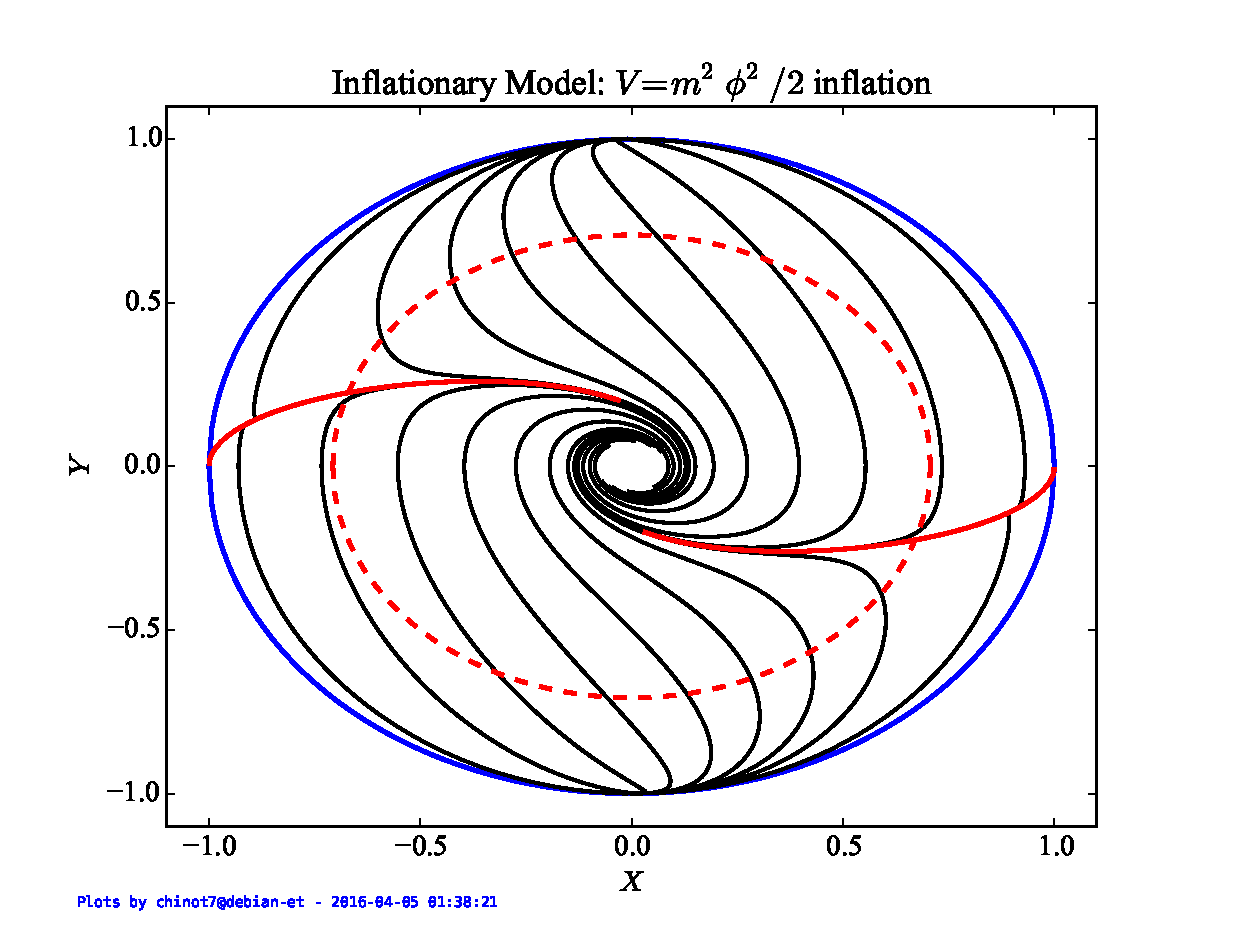
\includegraphics[scale=0.4]{../../Figures/Python_plots/Reheating_Dyn_Sys_python/Poincare_compact_dyn_sys/plots/phi2_phase_space_compactified_2D.eps}}
        \subfigure[]{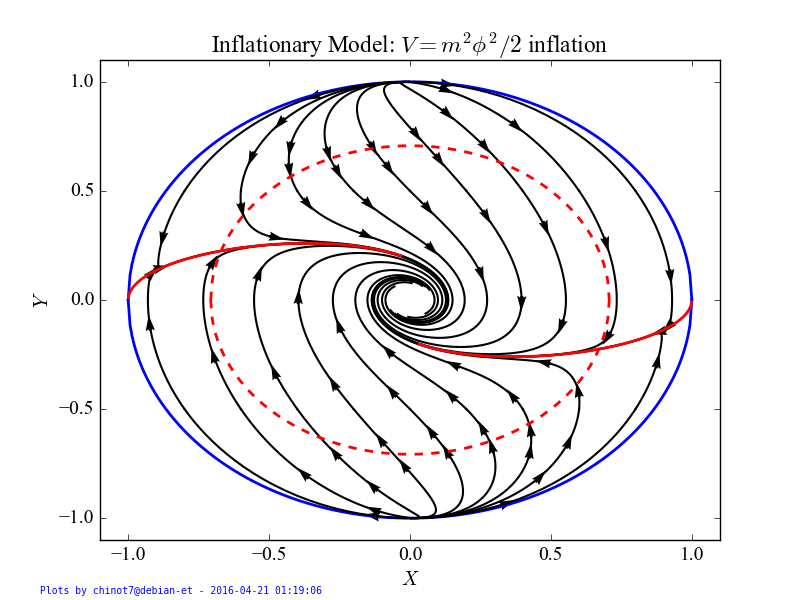
\includegraphics[scale=0.4]{../../Figures/Python_plots/Reheating_Dyn_Sys_python/Poincare_compact_dyn_sys_NEW/plots/phi2_phase_space_compactified_2D.png}}
        %\subfigure[]{\includegraphics[scale=0.4]{../../Figures/Python_plots/Reheating_Dyn_Sys_python/Poincare_compact_dyn_sys/plots/phi2_phase_space_compactified_3D.eps}}
        \subfigure[]{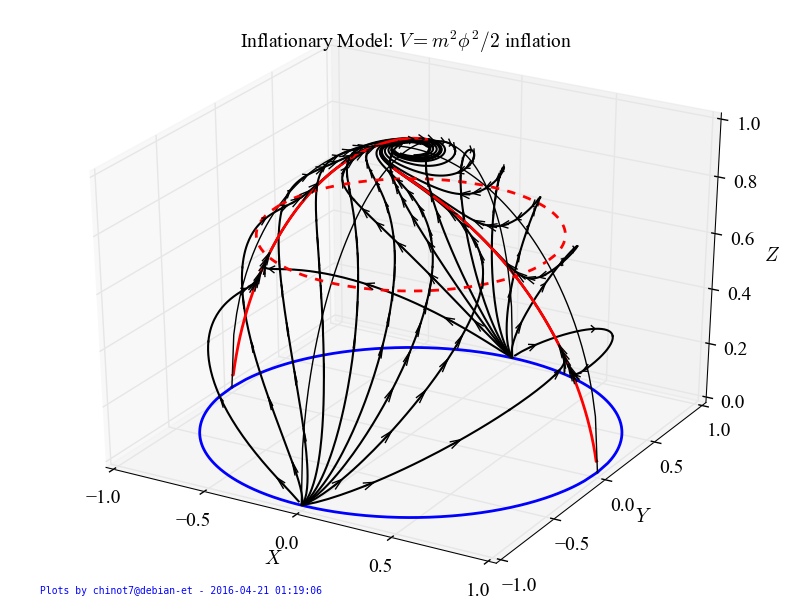
\includegraphics[scale=0.4]{../../Figures/Python_plots/Reheating_Dyn_Sys_python/Poincare_compact_dyn_sys_NEW/plots/phi2_phase_space_compactified.png}}
        \subfigure[]{\includegraphics[scale=0.4]{../../Figures/Python_plots/Reheating_Dyn_Sys_python/phi2_flow_near_critical_at_equator_Y=1.pdf}}
        \caption{\etcomment{Discuss the projection of on the Poincare sphere,
                here and the text.}Vector plot for the dynamical system given by
                 eqs.~\eqref{eq:dynamic_x}, \eqref{eq:dynamic_y} and
                 \eqref{eq:dynamic_z}. Several orbits with different initial
                 conditions are included (thick black lines). The two horizontal
                 red lines are the attractors, this shows that our estimation
                 $y_{atr}\sim \pm 1/3$ is in good agreement with the full
                 numerical solution. Even when the oscillations about the origin
                 that characterizes the graceful exit are present in every
                 orbited plotted not all give viable inflationary solution.
                 See the text for details.}
        \label{fig:full_x_y_dynamical_phase_space}
    \end{center}
\end{figure}



\begin{figure}[ht]
    \begin{center}
        \includegraphics[scale=0.7]{../../Figures/cosmomc_plots/ns_vs_r_PLANCK_vs_WMAP_from_PLA.pdf}
        \caption{\etcomment{Include this here?} WMAP (grey), PLANCK (with WMAP polarization data) (red) and
                 PLANCK + BAO (blue) bayesian constraints on the
                 inflationary parameters $n_s$ and $r$. The combination of
                 different sets of data strongly constraint the inflationary
                 predictions.}
        \label{fig:ns_vs_r_1}
    \end{center}
\end{figure}

\begin{figure}[ht]
    \begin{center}
    \includegraphics[scale=0.7]{../../Figures/cosmomc_plots/ns_vs_r_PLANCK_vs_WMAP_from_PLA_with_markers.pdf}
    \caption{PLANCK (with WMAP polarization data) (red) and PLANCK + BAO (blue)
             bayesian constraints on the inflationary parameters $n_s$ and $r$.
             The quadratic model predictions are marked for $N=40$ (green smaller
             point), $N=50$ (red mid point) and $N=60$ (lower blue point).}
    \label{fig:ns_vs_r_2}
    \end{center}
\end{figure}






%\begin{figure}[htbp]
%\begin{center}
%\includegraphics[scale=0.8]{../Figures/0907.5424v2/WMAP5_ns_r}
%\caption{{\bf default}}
%\label{default}
%\end{center}
%\end{figure}

%%\subsection{Dynamics of Inflation}

\section{Compactified solutions on the Poincare Sphere}





%
%%%%%%%%%%%%%%%%%%%%%%%%%%%%%%%%%%
\section{Reheating}
%%%%%%%%%%%%%%%%%%%%%%%%%%%%%%%%%%

In the last section we analyzed  the cosmological state at the end of inflation.
At that time the universe evolved as a cold and dust dominated universe. Even when
our discussion is restricted to $V\sim\phi^2$ model, it can be shown that this
conclusion is more general and shared with others chaotic..\footnote{A
    remarkable exception is \textit{thermal inflationary model}, where the
    inflaton decay is continuous during the inflation precess itself.}

In this scenario all energy is contained in the inflaton sector of fields
and, due to the exponential expansion, all other kind of particles had been
diluted. As a consequence, the inflaton must decay into other less massive fields
to increase the kinetic energy of the matter content. This  decay
process would be possible only if the inflaton is able to interact with other fields.
However, this interactions are unknown because the nature of the inflaton remains
hidden. 

In the next chapter we discuss the dynamics of reheating in the quadratic model
by  introducing simple interactions in the pure scalar sector. Contrary to the
transparent solutions obtained in inflation, the reheating dynamics are more
difficult to be analyzed because the non-linear phenomena determine the main
features of this reheating models.


%recover a proper Hot Big
%bang Model by the time of nucleosynthesis at $T\sim 1MeV$. In next chapter we
%analyse this reheating physics in more detail.


%\begin{figure}[htbp]
%\begin{center}
%\includegraphics[scale=0.8]{../../Figures/0907.5424v2/LargeField}
%\caption{{\bf default}}
%\label{default}
%\end{center}
%\end{figure}

%\begin{figure}[htbp]
%\begin{center}
%\includegraphics[scale=0.8]{../../Figures/0907.5424v2/SmallField}
%\caption{{\bf default}}
%\label{default}
%\end{center}
%\end{figure}

%
%%\subsection{The Universe at the end of inflation}
%
%
%%%%%%%%%%%%%%%%%%%%%%%%%%%%%%%%%%
%\section{Thermal History of the Universe}
%%%%%%%%%%%%%%%%%%%%%%%%%%%%%%%%%%
%
%
%
%\begin{table}[h!]
%\caption{Major Events in the History of the Universe.}
%\label{tab:timeline}
%\begin{center}
%\begin{tabular}{l | r | r | r}
% & {\small Time} & {\small Energy} & \\
% \hline
% \hline
% {\small Planck Epoch?} & {\small $< 10^{-43}$ s} & {\small $10^{18}$ GeV} &\\
% {\small String Scale?} & {\small $\gtrsim 10^{-43}$ s} & {\small $\lesssim 10^{18}$ GeV} & \\
%{\small Grand Unification?} & {\small $\sim 10^{-36}$ s} & {\small $10^{15}$ GeV} & \\
%{\small Inflation?} & {\small $\gtrsim 10^{-34}$ s} & {\small $\lesssim 10^{15}$ GeV} &\\
%{\small SUSY Breaking?} & {\small $< 10^{-10}$ s} & {\small $> 1$ TeV} &\\
%{\small Baryogenesis?} & {\small $< 10^{-10}$ s} & {\small $> 1$ TeV} &\\
%{\small Reheating?} & {\small $< 10^{-10}$ s} & {\small ?} &\\
%
%\hline
%\hline
%{\small Electroweak Unification} & {\small $10^{-10}$ s} & {\small 1 TeV} &\\
%{\small Quark-Hadron Transition} & {\small $10^{-4}$ s} & {\small $10^2$ MeV} &\\
%{\small Nucleon Freeze-Out} & {\small 0.01 s} & {\small 10 MeV} &\\
%{\small Neutrino Decoupling} & {\small 1 s} & {\small 1 MeV} &\\
%{\small BBN} & {\small 3 min} & {\small 0.1 MeV} &\\
%\hline
%\hline
%& & & {\small Redshift} \\
%\hline
%\hline
%{\small Matter-Radiation Equality} & {\small $10^4$ yrs} & {\small 1 eV} & {\small $10^4$}\\
%{\small Recombination} & {\small $10^5$ yrs} & {\small 0.1 eV} & {\small 1,100}\\
%{\small Dark Ages} & {\small $10^5 - 10^8$ yrs} & & {\small $> 25$} \\
%{\small Reionization} & {\small $10^8$ yrs} & & {\small $25 - 6$}\\
%{\small Galaxy Formation} & {\small $\sim 6 \times 10^8$ yrs} & & {\small $\sim 10$} \\
%{\small Dark Energy} & {\small $\sim 10^9$ yrs} & & {\small $\sim 2$} \\
%{\small Solar System} & {\small $8 \times 10^9$ yrs} & & {\small 0.5} \\
%{\small Albert Einstein born} & {\small $14 \times 10^{9}$ yrs} & {\small 1 meV} & {\small 0} \\
%\hline
%\end{tabular}
%  \end{center}
%\end{table}

%\begin{figure}[htbp]
%\begin{center}
%\includegraphics[scale=0.5]{../Figures/0907.5424v2/timeline}
%\caption{{\bf default}}
%\label{default}
%\end{center}
%\end{figure}
%
%
%\subsection{Bariogenesis}

%\subsection{Necleosinthesis}

%\subsection{Decoupling}

%\subsection{Radiation-Matter Transition}

%\subsection{$\Lambda$ - Dark Energy domination}

% ======================
\section{Appendix}
\label{sec:appendix}
% ======================

% ~~~~~~~~~~~~~~~~~~~~~~~~~~~
\subsection{Python Packages}
\label{sub:python_packages}
% ~~~~~~~~~~~~~~~~~~~~~~~~~~~

%\lstinputlisting[language=Python]{../../Codes/Python_Packages/cosmomodel.py}

%\begin{lstlisting}
%    x=1
%\end{lstlisting}


\bibliographystyle{plain}   % if natbib is available
%\bibliography{./bib/PBH_Biblio,./bib/supernova}
\bibliography{./bib/supernova}
%\end{comment}

\end{document}
%%%%%%%%%%%%%%%%%%%%%%%%%%%%%%%%%
